% *** LaTeX-mal for labrapporter i FY1001 Mekanisk fysikk, NTNU ***
% Jonas Tjemsland og Rolf Jonas Persson september 2021

% Basert på LaTeX-mal for labrapporter i FY1001, v.01.11.2011, og tidligere labhefter.

% Dette er et eksempel på et LaTeX-dokument, og du kan bruke dette som et utgangspunkt for 
% din egen rapport. Den enkleste måten å komme i gang med LaTeX er ved å benytte seg
% av Overleaf (https://www.overleaf.com) gjennom en nettleser. Dette krever ingen
% installasjon og flere personer kan redigere samme dokument samtidig.

% Her i starten og videre nedover i teksten under har vi lagt inn en god del linjer som starter med
% tegnet "%". Alt som kommer etter et slikt tegn på den linja er kommentarer og vil ikke synes i den 
% ferdige teksten. Vi bruker det for å forklare ting underveis. 

% Først må vi definere noen ting for dokumentet:

% Den første linjen i ethvert TeX-dokument definerer dokumentklassen. Dette gir en overordnet stuktur
% vi bygger dokmentet på. Noen vanlige klasser er "article", "report", "book", "slides" og "letter".
% Her skal vi bruke "elsarticle", som er dokumentklassen man må bruke om man ønsker å publisere
% i Elsevier-tidsskriftene.

\documentclass[5p]{elsarticle}
% I klammeparantesen kan vi definere noen parametere som er spesifikt for hver klasse.
% For eksempel gir "5p" 2 kolonner per side, og 1p gir 1 kolonne per side. Dette er spesifikt for elsarticle.

% Vi laster inn en del pakker i starten av dokumentet som inneholder kommandoer og miløer vi vil få bruk for.
\usepackage[utf8]{inputenc}                   % Mulighet til å skrive utf8-symboler
\usepackage[norsk]{babel}				      % Tilpasning til norsk
\usepackage{graphicx}       				  % For å inkludere figurer
\usepackage{amsmath,amssymb} 				  % Ekstra matematikkfunksjoner
\usepackage[font=small,labelfont=bf]{caption} % For justering av figurtekst og tabelltekst
\usepackage{hyperref}                         % For å skrive klikkbare linker

% Vi kan også definere egne funksjoner
\newcommand{\enhet}[1]{~\mathrm{#1}}  % Kommando for å enklere typesette enheter

% Gjør noen fornorskinger (vanligvis holder et med pakken "babel", men Elsarticle ødelegger)
% Endrer fra "Preprint submitted to" til "Preprint forelagt"
\usepackage{etoolbox}
\makeatletter\patchcmd{\ps@pprintTitle}{Preprint submitted to}{Preprint forelagt}{}{}\makeatother
% Abstract -> Sammendrag
\abstracttitle{Sammendrag} % Spesifikt for elsarticle

% Her skriver man tittel og forfatterinformasjon
\title{Mal for labrapport i FY1001 Mekanisk fysikk}
\author[fysikk]{T. C. Djupvik}
\author[fysikk]{O. F. Jakobsen}
\address[fysikk]{Institutt for fysikk, Norges Teknisk-Naturvitenskapelige Universitet, N-7491 Trondheim, Norway.}
\journal{Labveileder} % Leveres til labveileder

%%%%%%%%%%%%%%%%%%%%%%%%%%%%%%%%%%%%%%%%%%%%%%%%%%%%%%%%%%%%%%%%%%%%%%%%%
% Selve dokumentet befinner seg i miljøet "document". Et miljø starter med kommandoen "\begin{}" og ender med "\end{}".
% Vi kommer til å benytte oss av en rekke slike miljøer i dokumentet.
\begin{document}

\begin{abstract}
Denne teksten tar for seg hvordan man skriver en fysikkrapport. I tillegg fungerer
den som en mal for rapporten som skal skrives som en del av semesteroppgaven i emnet FY1001 – Mekanisk fysikk.

\textit{Her skriver du et sammendrag av rapporten. Sammendraget skal være veldig kort
men må inneholde svaret på tre spørsmål: 1. Hva gjorde du (hva målte du)? 2. Hvordan 
gjorde du det (hvilken metode)? 3. Hva fant du (resultat)?}
\end{abstract}

\maketitle % Denne kommanoden skriver ut dokumentinformasjonen, overskrift og sammendrag.

%%%%%%%%%%%%%%%%%%%%%%%%%%%%%%%%%%%%%%%%%%%%%%%%%%%%%%%%%%%%%%%%%%%%%%%%%
\section{Innledning}
Alle som deltar i vitenskapelig og teknisk arbeid, må i større eller mindre
grad kunne utforme en endelig skriftlig dokumentasjon av sine undersøkelser. 
Vitenskapelig arbeid dokumenteres i første omgang i form av en
laboratoriejournal eller kommentarer i kildekoder i numeriske programmer,
men dette er primærdokumenter som vanligvis
omhandler kun en del av en vitenskapelig eller teknisk undersøkelse og
er utformet med sikte på en begrenset leserkrets. Den endelige
dokumentasjonen av en undersøkelse er vanligvis i form av en rapport, en
tidsskriftartikkel eller en bok som er utformet med sikte på en stor
leserkrets. Denne er fullstendig og presenterer resultatene fra
undersøkelsen i en større sammenheng enn journalen, mens journalen i
større grad vil inneholde eksperimentelle detaljer. En forskjell er målgruppen, journalen er for deg og lab-medarbeidere, mens rapporten er for andre.

Det finnes ingen endelig fasit på hvordan en rapport skal være utformet, men
rapporter fra laboratorie\-under\-søkelser bør inkludere \emph{all vesentlig} informasjon
fra journalen i redigert form. I tillegg bør bakgrunnen for at undersøkelsen ble
satt i gang kommenteres. Det skal redegjøres for de teoretiske modeller som anvendes
i tolkningen av resultatene, og resultater fra teoretiske beregninger bør sammenliknes 
med de målte verdiene. Resultater fra tidligere undersøkelser bør omtales og
sammenliknes med de nye resultatene. Kvalitet, omfang og betydning av de nye resultatene
må vurderes i forhold til tidligere resultater. 
At det ikke finnes en ``fasit'' betyr ikke at man kan skrive hvordan man vil. Oftest finnes det en mal som man skal bruke. 

% Her benyttet vi oss av tegnet "\-". Dette hjelper LaTeX å velge hvor ord eventuelt kan bli delt opp

Dette dokumentet skal virke som en mal for rapportskriving i fysikk og som en generell
beskrivelse av hvordan man skriver tekster med ligninger på en ryddig måte. 
Malen skal benyttes i semesteroppgaven i emnet FY1001 -- Mekanisk fysikk.
Rapporten skal ha fire seksjoner i tillegg til sammendraget:
innledning, teori og metode, resultat, diskusjon og konklusjon.\footnote{
Merk at det ikke finnes en generell regel for hvordan kapittelutformingen skal være i en rapport.
For eksempel kan teori og metode skrives hver for seg, og man kan ha med en seksjon ``apparatur''.
}
Informasjon angående hva hver seksjon bør inneholde er beskrevet i kursiv i de respektive seksjonene.

%
% Merk at vi her bruker `` '' for å typesette anførselstegn (og ikke " "!). 
%

Det anbefales at \LaTeX~ brukes i utformingen av fysikkrapporten.
Dette er enerådende i mate\-matikk- og fysikkmiljøet når det gjelder 
skriving av litt tunge (og svært tunge) matematiske tekster. 
Prinsippet er omtrent som skriving av html-kode: Det skrives 
et dokument i reint tekstformat med kommandoer som deretter kjøres
gjennom en typesetter og dermed genererer et meget pent tekstbilde. 
Teksten du leser her er skrevet i \LaTeX.
Den enkleste måten å starte å bruke \LaTeX~ er ved å benytte seg av det
nettbaserte programmet \href{https://www.overleaf.com}{Overleaf}, laste råfilen (.tex) til 
dette denne malen opp, og kaste seg ut i skrivingen.
Overleaf krever ingen installasjon, og man kan jobbe flere personer på samme dokument samtidig.
Råfilen inneholder en del kommentarer som forklarer hvordan man skriver et \LaTeX-dokument.

% Kommandoen "\footnote" lager en fotnote og "\href" en klikkbar link.

\textit{I innledningen skal du forklare hensikten med rapporten, definere omfanget, gi grunnene til at undersøkelsen 
ble satt i gang og hvor den ble utført. Du skal forklare hvordan undersøkelsen fortsatte fra beslektet tidligere 
arbeid og sette den inn i en historisk sammenheng, noe som gjerne krever et lite litteraturstudium.
Dersom vi vil referere til kilder, f.eks. en lærebok \cite{goldstein} eller artikkel \cite{Weinberg:1967tq}
kan vi gjøre det som vist her. Referanselisten kommer til slutt i rapporten. Husk at kilder og referanser alltid
må komme tydelig frem når de er benyttet! Det finnes imidlertid mange ulike konvensjoner for hvordan disse skal
refereres til og listes opp.}

%%%%%%%%%%%%%%%%%%%%%%%%%%%%%%%%%%%%%%%%%%%%%%%%%%%%%%%%%%%%%%%%%%%%%%%%%
\section{Teori og metode}

\textit{Dette kapittelet skal beskrive den underliggende teorien som trengs for å forstå resultatene og metoden som er benyttet.
Vi bruker ordet metode i betydningen grunnleggende målemetode og ikke i betydningen detaljert fremgangsmåte. Dette gjelder
både numeriske beregninger og eksperimentelle metoder. Kapittelet bør derfor først og fremst inneholde en beskrivelse av
grunnleggende prinsipper. Detaljert beskrivelse av fremgangsmåten i laboratoriet, detaljerte utledninger av matematiske uttrykk
og forklaring av numerisk kildekode skal ikke være med i en rapport unntatt
når det har direkte betydning for resultatene.  Gjør rede for alle forutsetninger for bruk av teori og metode.
Begrunn valg av metode. Gi så mange detaljer om apparaturen og de numeriske metodene at en erfaren kollega kan gjenta
resultatene. Gi en prinsipiell analyse av apparaturens og metodens nøyaktighet. Beregnede tallverdier for målefeil
gis i resultatdelen.}

I teoridelen har man ofte behov for å skrive matematiske formler. Her kommer et eksempel på et par ligninger og hvordan vi kan referere til dem:

Svingetiden til en rektangulær pendel med uniform massefordeling kan uttrykkes som 
\begin{equation}
	T = 2\pi \sqrt { \frac{ r^2  + h^2 }{ gh } },
	\label{svingetid} % Labelen er det vi må huske når vi senere skal referere til ligningen.
\end{equation}
der $g=9,81\enhet{m/s^2}$ er tyngdens akselerasjon og $h$ er avstanden fra opphengningspunktet til massemiddelpunktet. Treghetsradien $r$ er gitt ved
\begin{equation}
	r = \sqrt {\frac{ l^2  + b^2 }{12} },
	\label{treghetsradius}
\end{equation}
der $l$ er lengden og $b$ er bredden til pendelen. Disse ligningene kan vi nå henvise til, for
eksempel kan vi si at vi skal bruke ligning \eqref{svingetid} til å måle tyngdeakselerasjonen $g$.

% Ligningsreferanser skal alltid være omsluttet av parenteser, og det ordnes automatisk
% når vi bruker kommandoen "\eqref{}". Hvis man ønsker en referanse uten parenteser, bruker man 
% kommandoen "\ref{}". Her kunne vi altså også ha skrevet "(\ref{svingetid})" 
% (men hvorfor gjøre det vanskelig?).

% Legg merke til at alle symbolene i ligningen står i kursiv. Bokstaver vil alltid stå i 
% kursiv når vi er i matematikkmodus. I et tekstavsnitt kan vi stille om til mattemodus ved å bruke
% dollartegn "$" som vi har gjort for tyngdeakselerasjonen g osv. i avsnittet over.

% Merk også at enheten er gitt i vanlig tekst ved hjelp av den egendefinerte kommandoen "enhet".
% Enheter og annen "vanlig" tekst skal som hovedregel ikke stå i kursiv.
% Her har vi også brukt kommandoen \SI fra siunitx-pakken for å presentere måltall og enheter på en 
% typografisk korrekt måte. Andre kommandoer er \num for (bare) tall og \si for (bare) enheter. For mer avansert bruk kan du søke opp "siunitx".

Legg merke til at vi har definert alle størrelser som inngår i ligningene. Videre kan vi merke oss at ligningene er
skrevet som en del av setningen, som gjør at teksten blir enkel å lese og flyter godt. Vi har altså avsluttet ligningene ovenfor med komma eller
punktum alt ettersom hva som passer for setningen som ligningene er en del av. Videre ser man at variabler (f.eks. $g$, $b$ og $l$) står i 
kursiv, mens enheter og vanlig tekst \emph{ikke} er i kursiv (f.eks. m, s).

Noen ganger trenger vi litt større oppstillinger av ligninger som går over flere linjer, og de kan se ut for eksempel som dette:
\begin{align}
	\left( \frac{\Delta r}{r} \right)^2 
	    &= \left( \frac{1}{r} \frac{\partial r}{\partial l} \Delta l \right)^2 
	        + \left( \frac{1}{r} \frac{\partial r}{\partial b} \Delta b \right)^2 \nonumber \\
		&=  \left( \frac{l \Delta l}{l^2 + b^2} \right)^2 + \left(\frac{b \Delta b}{l^2 + b^2} \right)^2.
\end{align}
Med det samme nevner vi at vi kan få bruk for subskript for å angi variabelnavn, for eksempel for å skille mellom $l_1$ og $l_2$.
Dersom subskriptet er et ord og ikke en indeks, må vi skrive variabelnavnet som for eksempel $l_\text{meterstav}$.
Merk at variabelnavnet ikke er i kursiv.

% Her har vi brukt align-miljøet til å sette ligningen opp over flere linjer. 
% Vi justerer likhetstegnene horisontalt ved å sette symbolet & foran dem.
% Kommandoen \\ brukes til å skifte linje. (Denne kan også brukes ellers i LaTeX, 
% men det anbefales som regel ikke. For å sørge for at bare en av linjene får 
% ligningsnummer, bruker vi kommandoen \nonumber for den første linjen.

%Noen ganger ønsker vi kanskje ikke ligningsnummer i det hele tatt. 
% (Men generelt ønsker vi at alle ligninger skal ha et ligningsnummer.)
%For eksempel vil vi nå kommentere i forbifarten at dersom $(l \Delta l)^2 \gg (b \Delta b)^2$ så får vi
%\begin{equation*}
%	\frac{\Delta r}{r} \approx \frac{\Delta l}{l}.
%\end{equation*}

%Her er vist et eksempel på en figur som vi henter inn fra en fil i PDF-format.
\begin{figure}[htb] 
% Alternativene inne i klammene angir hvilke av følgende plasseringer du vil tillate:
% h = here, t = top, b = bottom, p = separat, ! = forsøk å overstyre preferansene til LaTeX.
% (Preferansene til LaTeX gjør noen ganger at figurer ikke havner der du selv mener de passer best...).
  \begin{center}
      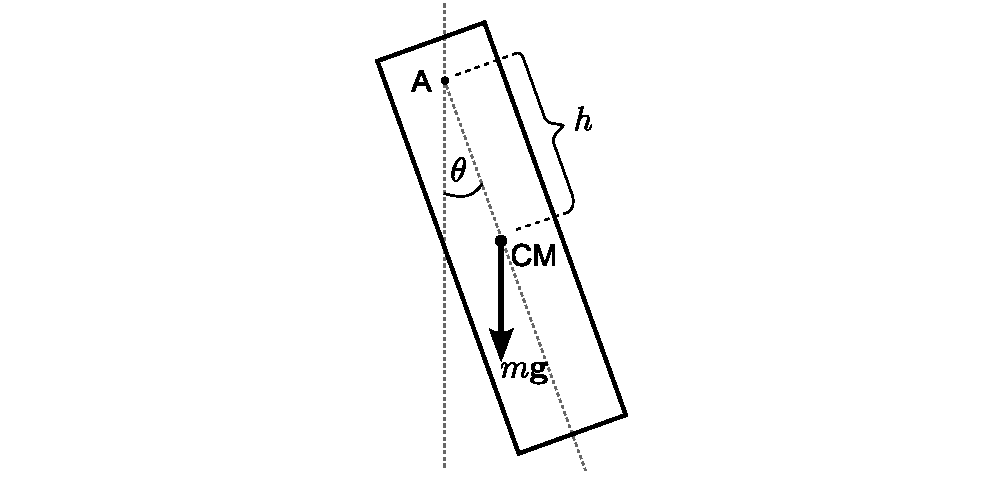
\includegraphics[width=0.3\textwidth]{pendel}  % Putter inn fila pendel.pdf
%   Hvis du angir bare enten width eller height, beholdes originalfigurens proporsjoner. (Dette anbefales.)
% 	Her har vi brukt width=0.3\textwidth for å angi figurbredde som en andel av den delen av arkbredden som inneholder tekst.
  \end{center}
  \caption{Her skriver du figurteksten. Merk at denne kommer under figuren. Naturligvis avslutter vi figurteksten med punktum,
  og det gjelder selv om den inneholder bare én setning eller til og med bare ett ord.}
  \label{MinLilleFigur} % Som med ligningen, er dette navnet vi refererer til.
\end{figure}

Vi kan referere til figurer på samme måte som vi refererer til ligninger. Nå refererer vi til 
figur \ref{MinLilleFigur}. Gode figurer skal være enkle ved at de begrenses til de forhold du
hovedsakelig ønsker å illustrere. De skal være klare ved at du bruker skarpe konturer, markere
symmetriakser vha.\ strek--punkt linjer (senterlinjer), markere snitt ved skravering, tydelige
målgrenselinjer og tydelige mållinjer med pilspisser og måltall. 
Figurer av mekaniske instrumentoppstillinger skal vise alle relevante romlige dimensjoner.
Vis tallverdier for romlige dimensjoner med mållinjer og måltall eller angi figurens målestokk.
Det er viktig at oppløsningen på figuren er tilstrekkelig til at alt er lett leselig og at teksten er stor nok.
Det beste er ofte å lage figurer i et vektorformat, slik som pdf. For enkle grafikker kan eventuelt png-format brukes.
% Legg merke til at nå bruker vi \ref{} og ikke \eqref{}. Figurreferansen skal ikke ha parenteser rundt seg.


%%%%%%%%%%%%%%%%%%%%%%%%%%%%%%%%%%%%%%%%%%%%%%%%%%%%%%%%%%%%%%%%%%%%%%%%%
\section{Resultat}

\textit{
Dette kapitlet er sterkt knyttet til laboratoriejournalen fra eksperimentet. Hvis du har skrevet en god journal og
fulgt anbefalinger om å gjøre alle tabeller og kurver ferdige under skriving av journalen, er resultatkapitlet lettskrevet. 
Prøv å gjøre det til et selvstendig kapittel. Presenter resultatene i logisk rekkefølge. Prøv også å legge resultatene frem
slik at de resultater som leder til konklusjonen trer klart frem. Bruk tabeller og diagrammer og angi resultater fra
eventuell feilanalyse av eksperimentet.  Hvis diskusjonskapitlet ser ut til å bli litt magert, kan det være en tanke å
kombinere resultatkapitlet og diskusjonskapitlet. Store sett med rådata hører ikke hjemme i en rapport, med mindre det er
presentert i en grafisk form.
}

Vi vil ofte skrive inn enkeltmålinger i resultatdelen, som at vi måler lengden til pendelen til å være\\
$l = 1000,015\pm0,005\enhet{mm}$, men dette kan også passe godt inn når metoden og aparaturen beskrives.
Kanskje vil vi skrive opp usikkerheten separat, som her er $\Delta l = 5\cdot 10^{-6}\enhet{m}$.

I denne delen har dere ofte bruk for tabeller. Et eksempel på dette kan du se i tabell \ref{MinLilleTabell}. 
Merk at denne tabellen inneholder få skillelinjer, som gjør at den blir ryddig og pen.
%
% Denne kan være litt vanskelig å forstå, men hvis du 
% studerer eksempelet nøye, blir det forhåpentligvis litt klarere.
%
\begin{table}[htb]
	\begin{center}
		\caption{Dette er den obligatoriske tabellteksten. Den kommer over tabellen.}
		\label{MinLilleTabell}	% Merkelappen vi vil referere til.
		\vspace{0.5cm}					% Litt ekstra plass for å få det til å se penere ut.
		\begin{tabular}{lll} 		% Tre venstrejusterte kolonner (l = left, c = center, r = right).
			\hline 								% Horisontal linje.
			$h$  &  $T$  & $g$  \\  			% Merk symboler i kursiv, (men det er fordi de er symboler, ikke fordi de er kolonneoverskrifter!)
			(cm) &  (s) & (m/s$^2$)\\ % mens enheter ikke er det.
			\hline												
			20   &  1,5744 & 9,836 \\
			23   &  1,5421 & 9,847 \\
			29   &  1,5229 & 9,839 \\
			33   &  1,5295 & 9,840 \\
			40   &	1,5637 & 9,829 \\
			\hline
		\end{tabular}
	\end{center}
\end{table}
% Litt ekstra forklaring av tabellen til slutt:
% Du skiller altså kolonnene med tegnet "&", og du setter inn linjeskift med "\\".
% (Dersom du får problemer med at kommaene ikke flukter i kolonnen, se kap. 8.3.1 i labheftet, eller bruk f.eks. pakken siunitx.)
% De horisontale linjene er plassert ifølge standarden du etterhvert bør ha begynt å bli vant til.

% Før man har lært seg å bruke LaTeX bør man ikke prøve å tvinge dokumentet til å se ut på en spesiell måte.
% En av de store fordelene med LaTeX er at man kan skrive teksten uten å tenke på dokumentformateringen. Denne er nemlig
% allerede satt opp for oss! LaTeX ordner alt av sideskift og bildeplasseringer for oss og det blir som regel bra dersom man har
% satt opp dokumentet rett.

Noen resultater kan også presenteres i form av diagrammer.
Tegn kun få kurver i hvert diagram. Forskjellige symboler kan brukes til å skille eksperimentelle punkter tatt opp under forskjellige 
betingelser. Vær imidlertid forsiktig med dette. Diagrammer hvor det blir tegnet mange kurver adskilt 
ved bruk av alt for mange forskjellige symboler blir fort uklare. 

\section{Diskusjon}
\textit{Her er det konklusjonen av resultatene dine som skal diskuteres, og
for å kunne diskutere dette må du sette dem inn i en større
sammenheng. Dette gjør du ved å relatere resultatene dine til
tidligere utførte undersøkelser på samme område, og ved å forutsi de
konsekvenser som resultatene av din undersøkelse medfører.}

%%%%%%%%%%%%%%%%%%%%%%%%%%%%%%%%%%%%%%%%%%%%%%%%%%%%%%%%%%%%%%%%%%%%%%%%%
\section{Konklusjon}
\textit{
Konklusjonen er rapportens viktigste del. I konklusjonen legger du frem ditt egentlige faglige bidrag. Det er som regel formidlingen av dette bidraget som er hovedgrunnen til at du skriver rapporten. Konklusjonskapitlet bør ikke skrives før du har tenkt grundig over resultatene fra dine egne målinger og sammenlignbare målinger gjort av andre i lys av den teori du har valgt å tolke resultatene innenfor. En god konklusjon er kort og presis, og presenterer kun hovedresultatet og konklusjonen fra diskusjonen. Eventuelt fremtidig arbeid kan også nevnes her. 
}

Vi har gitt dere et eksempel på rapportoppsett. Nå er det din tur -- lykke til!

%%%%%%%%%%%%%%%%%%%%%%%%%%%%%%%%%%%%%%%%%%%%%%%%%%%%%%%%%%%%%%%%%%%%%%%%%

% Her kommer referanselisten. Dersom du ønsker flere enn noen få referanser, kan det lønne seg å 
% søke opp "BibTeX" og sette seg litt inn i det. 
\begin{thebibliography}{99}	% Denne referanselisten kan ikke ha flere enn 99 referanser.

\bibitem{goldstein} % I klammeparentes angir vi merkelapp for de ulike oppføringene i listen.
H. Goldstein, C. P. Poole, og J. L. Safko. Classical Mechanics. Addison-Wesley, 3rd ed., June 2001.

\bibitem{Weinberg:1967tq}
S.~Weinberg,
%``A Model of Leptons,''
Phys. Rev. Lett. \textbf{19} (1967), 1264-1266
doi:10.1103/PhysRevLett.19.1264


\end{thebibliography}

\end{document}